\newpage
\section{Klassifikation partieller Differentialgleichungen}
\setcounter{equation}{0}
Erinnerung: Methoden der Charakteristiken zur Lösung pDgl.
\begin{bsp} 
Gesucht ist $x(z,t) \quad z,t,x \in \R$
\begin{align*} 
&(1+x)\frac{\partial x}{\partial t}-(1+z)\frac{\partial x}{\partial z} = z - t \\
\leftrightarrow&(1+x)\frac{\partial x}{\partial t}-(1+z)\frac{\partial x}{\partial z}  -z + t = 0
\end{align*}
Ansatz: $z=z(s)$, $t=t(s)$, $x=x(s)=x(z(s),t(s))$
Es gilt:
\begin{align*} 
&\frac{\d x}{\d t} = \frac{\partial x}{\partial z}\frac{\d z}{\d s} +\frac{\partial x}{\partial t}\frac{\d t}{\d s}  \\
\leftrightarrow & \frac{\partial x}{\partial z}\frac{\d z}{\d s} +\frac{\partial x}{\partial t}\frac{\d t}{\d s} - \frac{\d x}{\d t} = 0
\end{align*}
\textcolor{red}{Markieren in beiden Gleichungen, wass gleichgesetzt wird}

Offenbar muss gelten:
\begin{align*}
\frac{\d t}{\d s} &= 1+t \\
\frac{\d z}{\d s} &= -(1+z) \\
\frac{\d x}{\d s} &= z-t
\end{align*}
Dieses Gls. nennt man charakteristisches Dgl. System
Lösung (charakteristische Kurven):
\begin{align*}
t(s) &= C_1 e^s -1 \\
z(s) &= C_2 e^{-s} - 1 \\
x(s) &= C_3-C_2 e^{-s} - C_1 e^s \\
\end{align*}
Es gilt: 
\begin{align*}
e^s &= \frac{t+1}{C_1} = \frac{C_2}{z+1} \\
&\leftrightarrow (t+1)(z+1) = C_1C_2=:C \\
\end{align*}
ferner:
\begin{align*}
&x = C_3 - (z+1)-(t+1) \\
&x+z+t = C_3-2=: d \\
\end{align*}
Eine Lösung:
\begin{align*}
x(z,t)=-z-t+d \\
\end{align*}
Allgemein: $x = \phi((z+1)(t+1),x+z+t)$ ist Lösung mit beliebiger $\underbrace{C^1}_{\text{1-mal stetig diffbar}}$-Fkt. $: \phi:\R^2 \rightarrow \R$
\end{bsp}
\subsection{Charakteristika von Gleichungen erster Ordnung}
Ausgangspunkt:
\begin{align}
\label{eq:allgpde}
a(x(z,t),z,t)\frac{\partial x(z,t)}{\partial z}+b(x(z,t),z,t)\frac{\partial x(z,t)}{\partial t}=c(x(z,t),z,t)
\end{align}
Dabei ist $x$ eine Größe nach der aufgelöst werden muss.
Für eine beliebige Kurve
\begin{align*}
\Gamma: s \mapsto (z,t) = (a(s),b(s))
\end{align*}
wird eine Lösung von \eqref{eq:allgpde} vorgegeben:
\begin{align}
\label{eq:pdesolve}
x(a(s),b(s))=h(s)
\end{align}

\begin{figure}[ht]
	\centering
	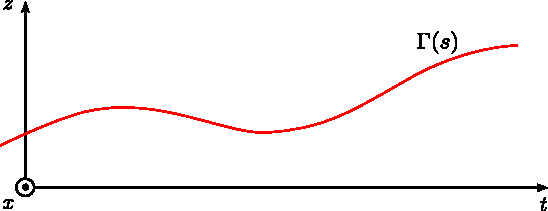
\includegraphics{img/charakteristik}
	\label{fig:charakteristik}
\end{figure}
Frage: Berechnung der Ableitungen $\frac{\partial x(z,t)}{\partial z}$ und $\frac{\partial x(z,t)}{\partial t}$ auf $\Gamma$ aus $h$ möglich?

Vorgehen: Differenzieren von \eqref{eq:pdesolve} nach $s$

\begin{align*}
\frac{\d h(s)}{\d s} = \frac{\partial x(z,t)}{\partial z}(\alpha(s),\beta(s))\alpha'(s)+\frac{\partial x(z,t)}{\partial t}(\alpha(s),\beta(s))\beta'(s)
\end{align*}
Zusammen mit \eqref{eq:allgpde} folgt:
\begin{align}
\label{eq:matrixpde}
\underbrace { \begin{pmatrix} a & b \\ \alpha ' & \beta ' \end{pmatrix} }_{ { \bm{C}} } \begin{pmatrix} \frac { \partial x }{ \partial z }  \\ \frac { \partial x }{ \partial t }  \end{pmatrix}=\begin{pmatrix} c \\ h' \end{pmatrix}
\end{align}
Kann nicht aufgelöst werden (Matrix nicht regulär), nennt man die Kurve $\Gamma$ charakteristisch.

Prüfung der Singularität von $\bm{C}$ wenn Zeilen linear abhängig sind
\begin{align}
\label{eq:singularitaetpruefung}
\alpha'= \frac{\d z}{\d s} = f_d a \big|_\Gamma \qquad \beta'= \frac{\d t}{\d s} = f_db \big|_\Gamma
\end{align}
mit der beliebigen Funktion $f_d$.
\begin{defi}
Eine nichttriviale Kurve $\Gamma:s\mapsto(\alpha(s),\beta(s)) \in \R^2$ heißt charakteristische Projektion zur pDgl. \eqref{eq:allgpde}, wenn \eqref{eq:singularitaetpruefung} mit einer beliebigen Funktion $f_d$ gilt.
\end{defi}
Charakteristiken:

Differenz der Zeilen von \eqref{eq:matrixpde} ergibt:
\begin{align*}
\frac{\d x}{\d s}\Big\rvert_\Gamma = h'= fc\big|_\Gamma
\end{align*}
Lösung der Kurve $\Gamma$ (entlang der Projektion) genügt der Dgl.
Es folgt mit \eqref{eq:singularitaetpruefung} das charakteristische Dgl.-System zu \eqref{eq:allgpde} ($f_d = 1,$ da beliebig):
\begin{align}
\label{eq:charkteristiken}
\frac{\d z}{\d s} = a \quad \frac{\d t}{\d s} = b \quad \frac{\d x}{\d s} = c
\end{align}
Lösungen $s \mapsto (t,z,x)$ des charakteristischen Systems \eqref{eq:charkteristiken} heißen charakteristische Kurven zu \eqref{eq:allgpde}.